\section{Proposed Research}
\label{sec:proposed-work}
%%

\subsection{Specific Aim 1: Measuring material properties of amphiphile
  self-assembly}
\label{subsec:specific_aim_1}

The proposed research aims to provide fundamental insight into the
self-assembly dynamics of amphiphilic particles. These results will
facilitate optimal design of smart materials by tuning the geometry and
properties of the amphiphilic particles.  Specific Aim 1 achieves this
through a novel mathematical model for particle self-organization driven
by long-range interfacial forces. 

\subsubsection{Problem formulation}
%\begin{wrapfigure}[h!]
\begin{wrapfigure}[10]{r}{0.55\textwidth}
  \centering
  \vspace{-12pt}
  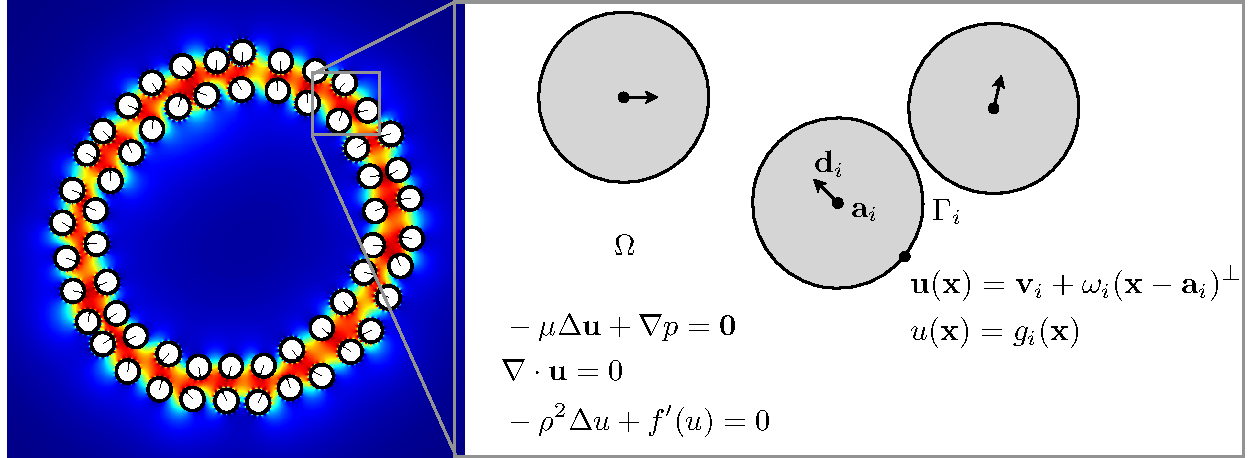
\includegraphics[width=0.55\textwidth]{figures/SpecificAim1/Domain.pdf}
  \caption{\label{fig:flow_map} A collection of amphiphilic particles
  suspended in a solvent. The solvent velocity satisfies the Stokes
  equations, and the hydrophobic forces depend on the solvent activity
  that satisfies the screened Laplace equation. The geometry is updated
  by solving the mobility problem.}
\end{wrapfigure}

The mathematical formulation is a nonlinear system for the dynamics of a
collection of particles. The interactions come from a system of linear
partial differential equations (PDEs) and comprise hydrodynamic
interactions and hydrophobic interactions.
%The formulation prevents particle collisions through excluded volume
%potentials. 
The hydrodynamic interactions come from the mobility problem for rigid
particles immersed in a viscous solvent, which we solve with a
second-order Adams-Bashforth method. Assuming inertial terms are
negligible, the particle motion is goverened by the Stokes equations
\begin{subequations}
  \label{eq:stokes}
  \begin{alignat}{3}
  \label{eq:stokes1}
  -\mu \Delta \uu + \nabla p &= \mathbf{0}, && \xx \in \Omega, \\
    \label{eq:stokes2}
  \nabla\cdot \uu &= 0, \qquad && \xx \in \Omega, \\
\label{eq:stokes3}
  \uu - \uu_\infty &\to \mathbf{0}, && |\xx| \to \infty,
  \end{alignat}
\end{subequations}
%\begin{alignat}{3}
%\label{eq:stokes1}
%  -\mu \Delta \uu + \nabla p &= \mathbf{0}, 
%    && \xx \in \Omega, \\
%\label{eq:stokes2}
%  \nabla\cdot \uu &= 0, \qquad && \xx \in \Omega, \\
%\label{eq:stokes3}
%  \uu - \uu_\infty &\to \mathbf{0}, && |\xx| \to \infty,
%\end{alignat}
%
where $\uu$ is the velocity and $p$ is the pressure of the solvent,
$\uu_\infty$ is the background flow, and $\mu$ is the constant solvent
viscosity. The domain $\Omega$ is the fluid region surrounding the
particles. Since the particles are rigid, the solvent velocity satisfies
a no-slip boundary condition for a rigid body motion 
%\begin{align}
%\label{eq:rigid_bc}
%  \uu(\xx) = \vv_i + \omega_i  (\xx - \aa_i)^\perp, \quad
%    \xx \in \Gamma_i,\qquad  i=1,\ldots,N_p,
%\end{align}
on the particle boundary $\Gamma_i$ with translational velocity $\vv_i$
and angular velocity $\omega_i$. Given imposed forces acting on each
particle, the \emph{mobility problem} consists of finding
translational and angular velocities so that viscous fluid forces
balance the imposed forces.

The hydrophobic interactions come from the tendency of particles to
minimize the free energy of the structure of the surrounding water
molecules. Experimental measurements suggest that the free energy
functional take the form 
\begin{align*}
\label{eq:free_energy}
  F[u] = C \int_{\Omega} \left(\rho |\nabla u|^2 + \rho^{-1} f(u)\right)
  \,d\xx,
\end{align*}
where $u$ is an order parameter for the structure of water, $\rho$ is a
decay length, $C$ is a constant, and $f(u)$ is a potential.
Hydrogen-bond persistence times are on the order of picoseconds
\cite{MaGa13}. Since waters reorient on a time scale much smaller than
the particle motion, $u$ minimizes $F[u]$ at all time, and therefore
satisfies 
\begin{equation}
\label{eq:SL}
-\rho^2 \Delta u + f'(u) = 0  \text{ in } \Omega,\quad u = g,
\text{ on } \bd\Omega.
\end{equation}
The boundary condition $g$ is a material label that is transported with
the particle motions (Figure~\ref{fig:bcs}).

\begin{wrapfigure}[10]{r}{0.65\textwidth}
  \vspace{-22pt}
  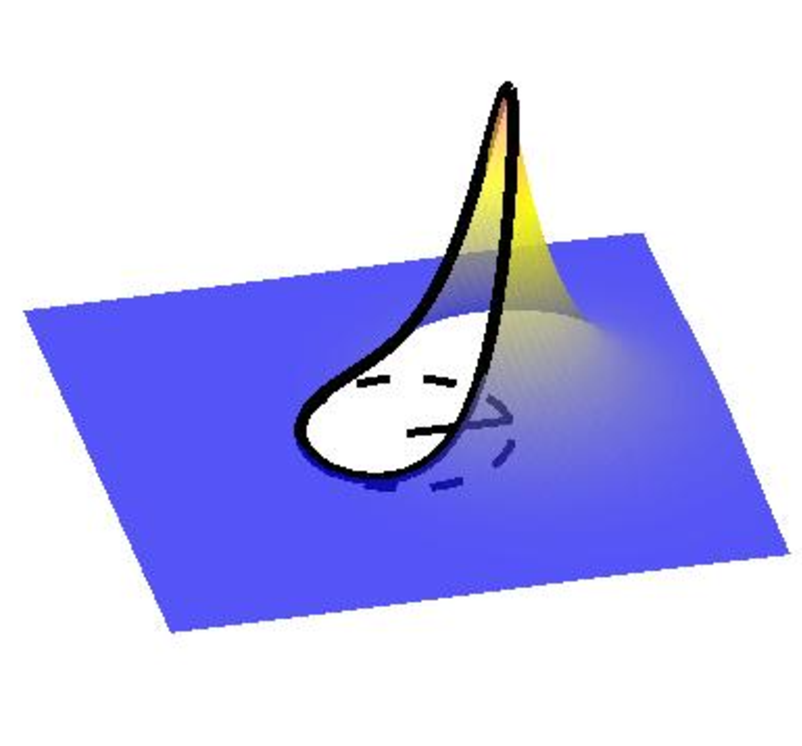
\includegraphics[width=0.2\textwidth]{figures/SpecificAim1/LPA.pdf}
  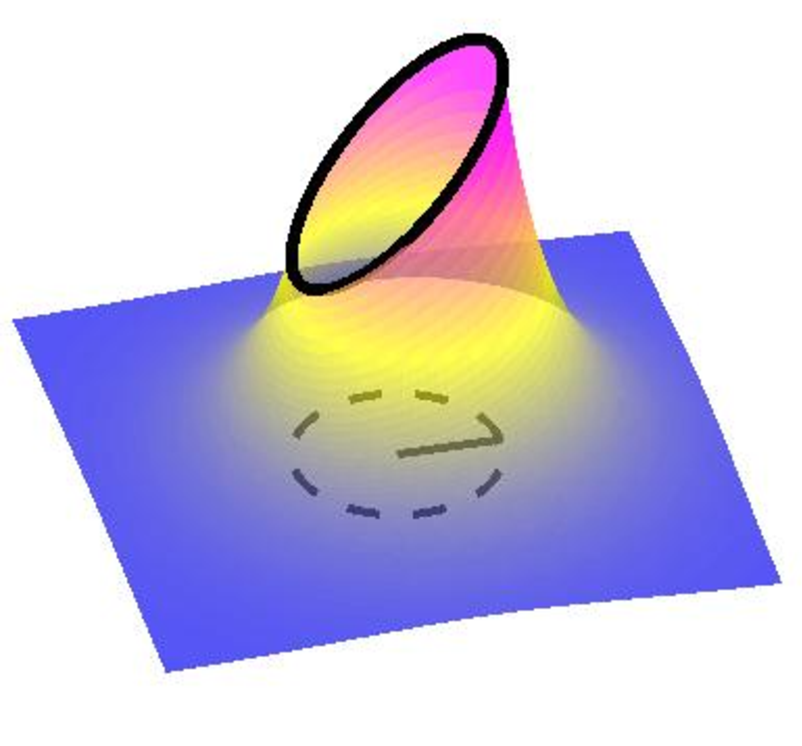
\includegraphics[width=0.2\textwidth]{figures/SpecificAim1/LPB.pdf}
  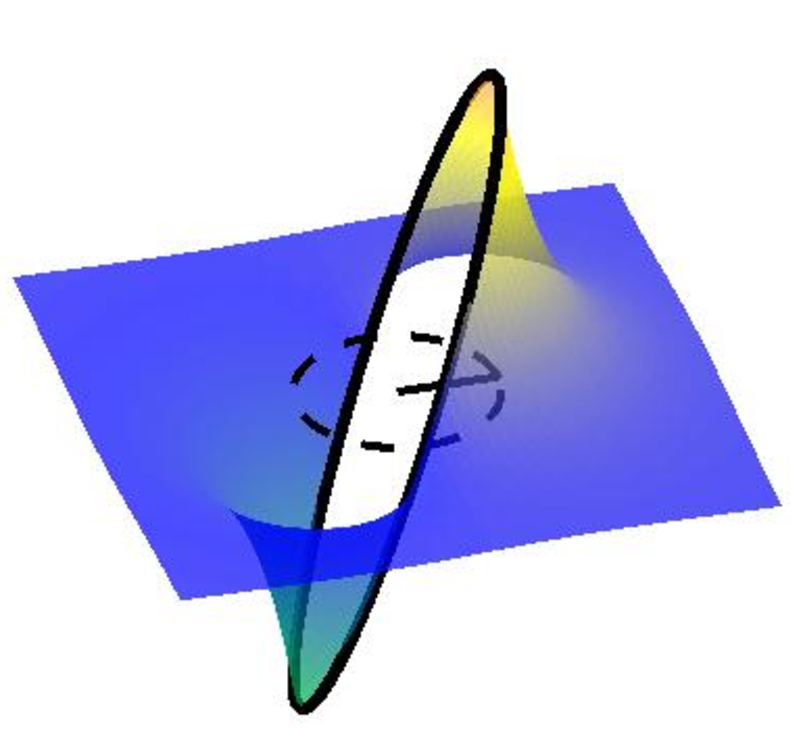
\includegraphics[width=0.2\textwidth]{figures/SpecificAim1/LPC.pdf}  
\caption{\label{fig:bcs} Boundary conditions characterize the type of
  water structure: an amphiphilic particle (left), a hydrophobic
  particle with anisotropic intensity (middle), a water structure with
  plus/minus polarity (right). The dashed curve is the boundary of the
  disk and the arrow its director.}
\end{wrapfigure}
The coupling between the Stokes equations \eqref{eq:stokes} and the
semilinear elliptic equation \eqref{eq:SL} comes from the first
variation of the energy functional. The particles minimize the free
energy $F[u]$ by altering the location of hydrophobic interfaces. It is
possible to calculate the rate of change of $F[u]$ using variation of
the domain~\cite{Bandle2015, Schiffer1954, Grinfeld2010}. Carrying out
this variation yields a 
%The hydrophobic forces are torques are
%\begin{equation}
%  \label{eq:hydrophobicAttraction}
%  \FF_i^{\text{hydro}} = \int_{\Gamma_i} {\bf T}\cdot \nnu \, \dif s, 
%    \quad 
%    T_i^{\text{hydro}} = \int_{\Gamma_i} (\xx - \aa_i)^{\perp} \cdot
%    ({\bf T} \cdot \nnu) \dif s.
%\end{equation}
surface force density 
\begin{align}
  \label{eq:stress}
\mathbf{T}
= C \left[ \rho^{-1} f(u) \mathbf{I}
  + \rho \left(|\nabla u|^2 \mathbf{I} - \nabla u \nabla u^T\right)\right].
\end{align}
The imposed forces and torques from the integration of $\mathbf{T}$
along the particle boundary. The density~\eqref{eq:stress} was first
introduced by~\cite{Fu2018_SIAM} and is the higher-dimensional analogue
of disjoining pressure calculated by \cite{MaRa76, ErLjCl89, KoNa15,
Nagle17, KUZMIN2005}. It is the mathematical ingredient responsible for
forming particle aggregates that sequester their hydrophobic surface
regions.

%By solving the above system, we obtain translational and angular
%velocities of the many-body system. A second-order Adams-Bashforth
%scheme updates the particle positions and orientations.

The formulation presents a number of mathematical and numerical
challenges. For one, the domain is constantly changing so that a new
boundary value problem must be solved at each time step.  The particle
boundaries are nearly touching and this requires high-order numerical
schemes to accurately calculate forces and adaptively chose an
appropriate time step size. Furthermore, there are issues with
accurately capturing the far-field boundary conditions in the unbounded
domain. Finally, the numerical routine must handle large system sizes
efficiently when their are many particles is large. 

%and
%\begin{equation}
%  \label{eq:force}
%  \int_{\Gamma_i} \ssigma \cdot \nnu \, \dif s = \FF_i,\quad 
%  \int_{\Gamma_i} (\xx - \aa_i)^{\perp} \cdot (\ssigma \cdot \nnu) \,
%  \dif s = T_i, \qquad i=1,\ldots,N_b,
%\end{equation}
%where
%$\ssigma = -p \mathbf{I} + \mu \left(\nabla \uu + \nabla \uu^T \right)$
%is the hydrodynamic stress tensor (pressure tensor) and $\nnu$ is the
%particle outward normal.

\subsubsection{Janus-particle self-assembly} 
When $f(u) = u^2$, and the water structure has its lowest potential
value at $u=0$ which represents bulk water. The solutions of
\eqref{eq:SL} have a boundary layer structure and decay to $0$ in the
bulk with the decay length $\rho$. Even in this linear response case, a
number of morphologies arise by altering boundary conditions.

\begin{figure}[h!]
  \begin{center}
    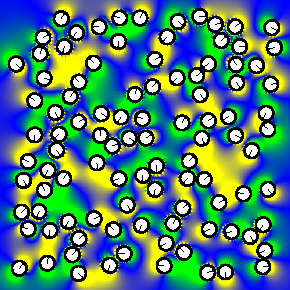
\includegraphics[width=0.32\textwidth]{figures/SpecificAim1/N100A1.pdf}
    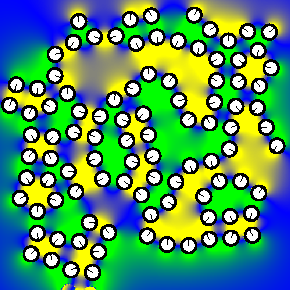
\includegraphics[width=0.32\textwidth]{figures/SpecificAim1/N100A2.pdf}
    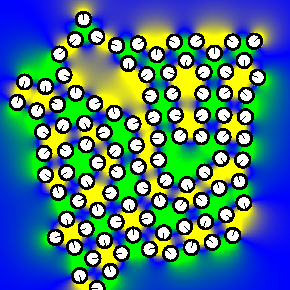
\includegraphics[width=0.32\textwidth]{figures/SpecificAim1/N100A3.pdf}
    \end{center}
  \caption{\label{fig:self-assemblyA} Self-assembly with a polar
  boundary condition leads to a checkerboard pattern. Green is for $u <
  0$, yellow is for $u > 0$, and blue is for $u = 0$.}
\end{figure}

Consider a polar boundary condition where $g_i(\xx) = (\pi r)^{-1/2}
\cos (\theta_i(\xx))$ where $\theta_i$ is the angle formed by $\xx$, the
particle center $\aa_i$, and the particle director $\dd_i$. The
normalization $(\pi r)^{-1/2}$ and others below provide a uniform
surface energy $\int_{\Gamma_i} g_i^2 \,ds = 1$ for circular particles
of radius $r$. The boundary condition is odd along the particle axis
making the particle head repel the tail.  We simulate the dynamics of
100 particles with random initial position and orientation. The
particles rapidly form chains with their directors perpendicular to the
length of the chain. The equilibrium structure consists of particles
positioned on a square grid in a checkerboard pattern
(Figure~\ref{fig:self-assemblyA}. This patterning is a consequence of
energy minimality and allows each particle to simultaneously coordinate
its head with the head of three other particles and its tail with the
tail of three other particles. 

\begin{figure}[h!]
\begin{center}  
    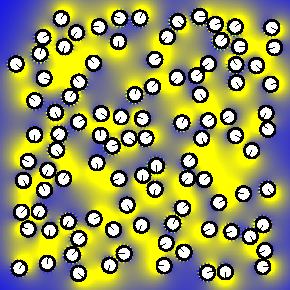
\includegraphics[width=0.32\textwidth]{figures/SpecificAim1/N100B1.pdf}
    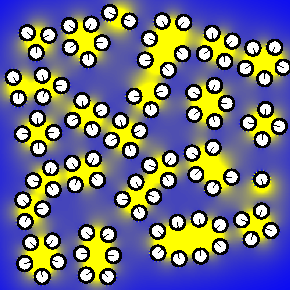
\includegraphics[width=0.32\textwidth]{figures/SpecificAim1/N100B2.pdf}
    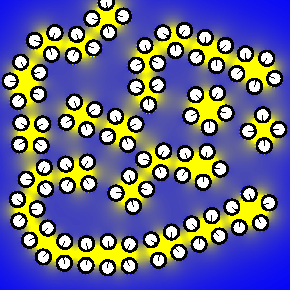
\includegraphics[width=0.32\textwidth]{figures/SpecificAim1/N100B3.pdf}
\end{center}    
  \caption{\label{fig:self-assemblyB} Self-assembly with with boundary
  condition that results in hydrophobic tails and hydrophilic heads. The
  resulting bilayer pattern shields the hydrophobic core (yellow) from
  the aqueous phase.}
\end{figure}
Amphiphilic particles have a hydrophobic tail and a hydrophilic head and
are accounted for as follows. The hydrophilic side takes the value $u =
0$ since the apolar head of a lipid, for example, does not alter
the structure of adjacent waters. The hydrophobic side takes the value
$u > 0$. The interaction between particles is attractive. Using $(3\pi
)^{-1/2}(1 + \cos(\theta_i(\xx)))$ as a simple modification to
the previous boundary condition produces two-dimensional micelles and
bilayers \cite{Fu2018_SIAM} (Figure~\ref{fig:self-assemblyB}).
Researchers have asked us if the phenomenon is robust. To show that it
is, we instead use the boundary condition
\begin{equation}
\label{eq:vonMises}
  g_i(\xx) = \sqrt{
  \frac{\exp( \kappa_i(\theta_i(\xx) - \theta^0_i))}
  {2\pi r_i I_0(\kappa_i)}}
\end{equation}
where the radicand \todo{radicand?} is the von Mises distribution with
director angle $\theta^0_i$ and Bessel function $I_0$ of order zero. The
square of this function behaves as a normal distribution with variance
like $1/\kappa_i$.To replicate experimental conditions, the
concentration $\kappa_i$ and radii $r_i$ are randomized. Using the same
initial configuration, the particles form small groups that
combine to form bilayers (Figure~\ref{fig:self-assemblyC}.


\begin{figure}[h!]
  \begin{center}
    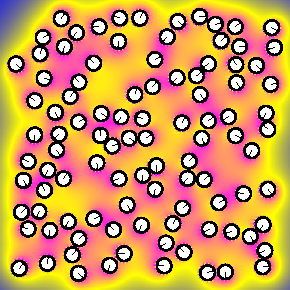
\includegraphics[width=0.32\textwidth]{figures/SpecificAim1/N100C1.pdf}
    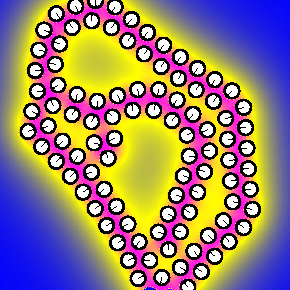
\includegraphics[width=0.32\textwidth]{figures/SpecificAim1/N100C2.pdf}
    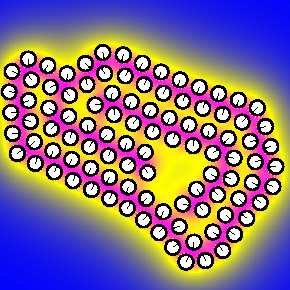
\includegraphics[width=0.32\textwidth]{figures/SpecificAim1/N100C3.pdf}\\
    \caption{Hydrophobic particles with a bias. The hydrophobic
    intensity is greater on one side of the particle (magenta) than the
    other (yellow).
    \label{fig:self-assemblyC}}
\end{center}
\end{figure}

Multilamelar bilayers arise with an increase by shifting the boundary condition
further. Let $g_i(\xx) = (9\pi )^{-1/2}(2 + \cos(\theta_i(\xx)))$.
This gives a hydrophobic particle with greater intensity of hydrophobicity
at $\theta_i = 0$ than at $\theta_i = \pi$.  The initial self-assembly
is similar to that of the amphiphilic particle case, except that the bilayers
do not stay well separated.  Rather, the bilayers stack on top of each
other as a consequence of the interfacial tension of exposed particle heads \cite{deMeetal21}. 

In summary, the hydrophibic interaction-mobility problem model yields
rich morphologies that are valuable in the synthesizing multiphasic and
anisotropic colloids \cite{Bradley2016,Mallory2017,Bradley2017}.
The main experimental challenges include the ability to
decouple particle surface properties.
The goal is to obtain numerically aided 
syntheses and assembly of soft matter materials.
Applications in this area include cargo-carrying capacity, 
catalytic activity, or stimuli-responsive shape-change to amplify colloid
utility for a wide range of  spanning environmental remediation to drug
delivery \cite{McBr21, HaBr20}.







%\begin{wrapfigure}[14]{l}{0.5\textwidth}
%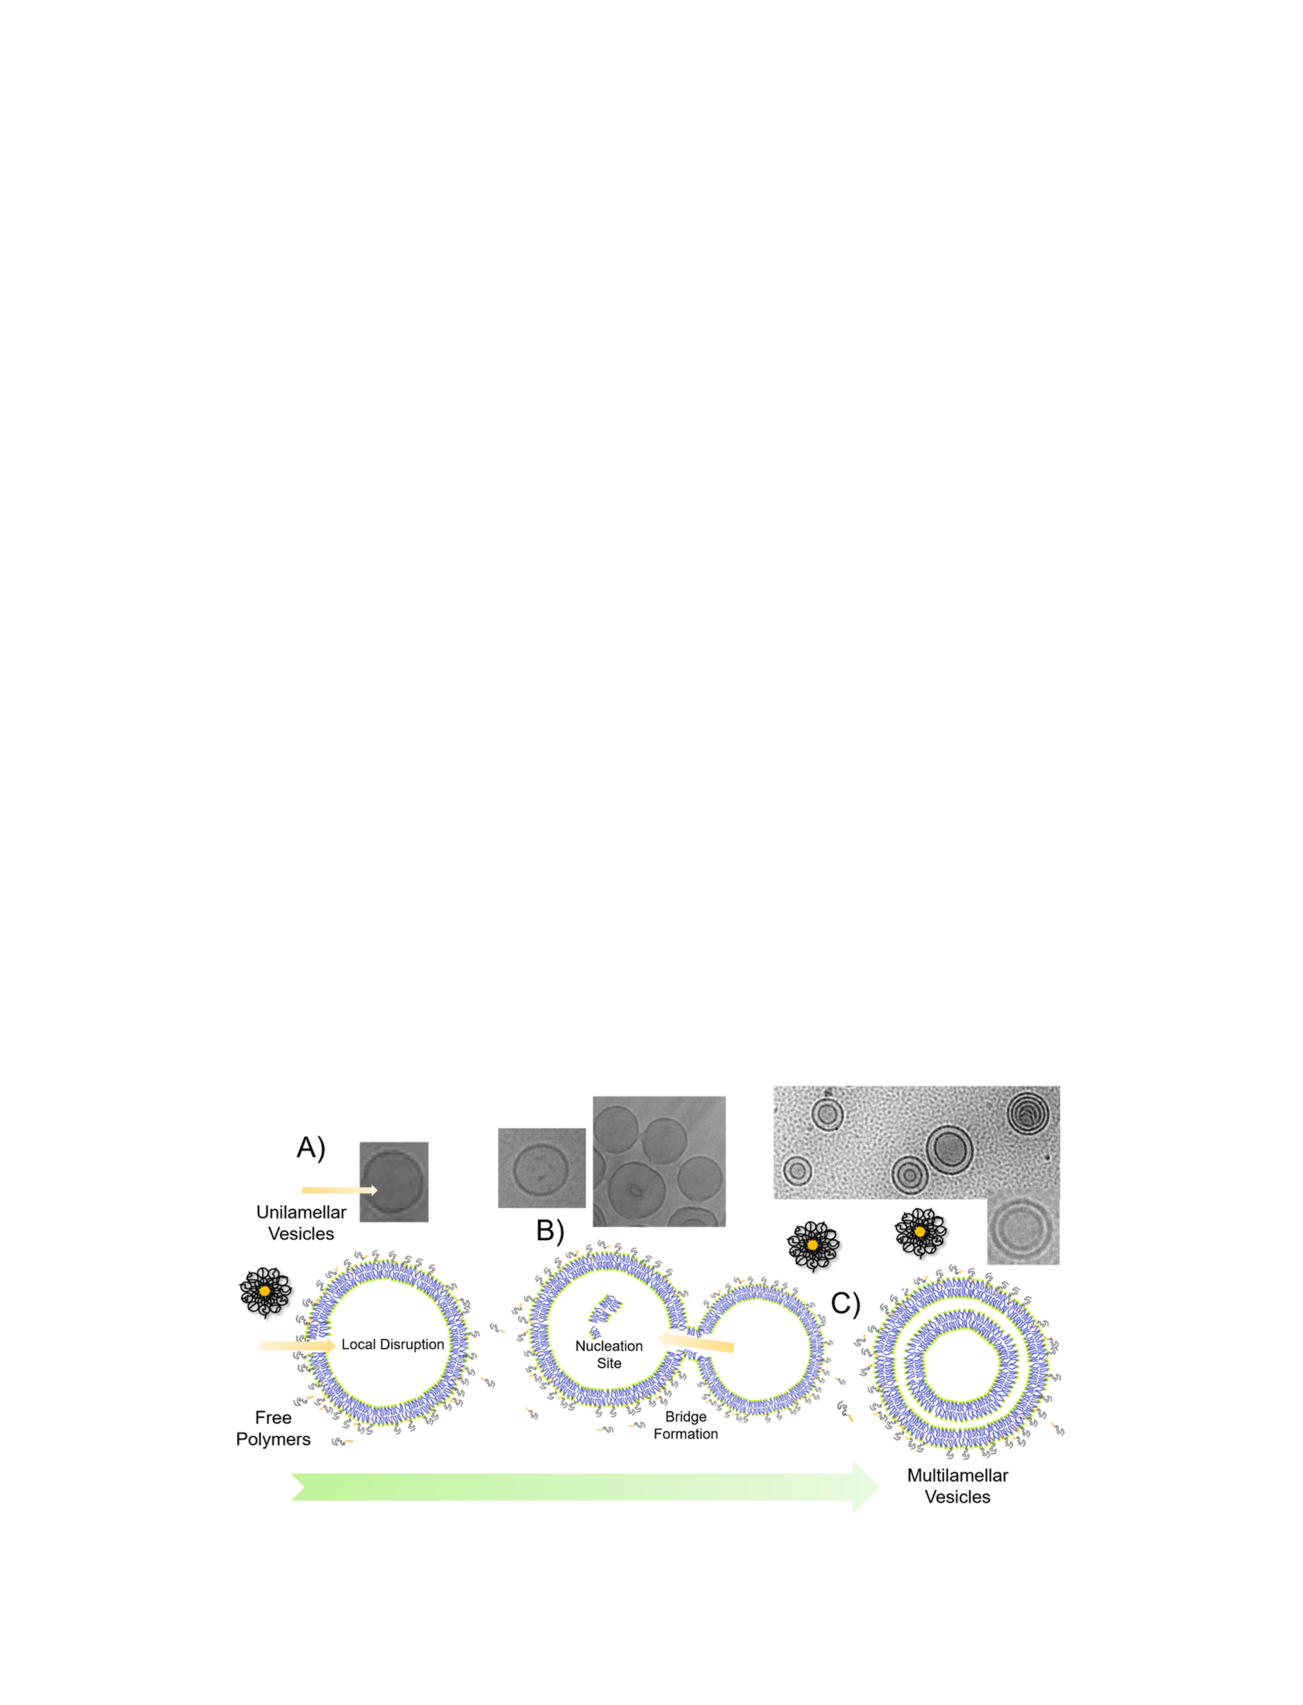
\includegraphics[width=0.5\textwidth]{figures/SpecificAi%m1/multilamelar.pdf}
%\caption{\label{fig:multilamelar}
%  Experimentalists can transform unilamellar vesicles to% multilamellar
%  vesicles by altering the quality of the solvent
%    \cite{deMeetal21}.
%  In \eqref{eq:SL}, the solvent quality enters through t%he potential
%  $f(u)$ and boundary conditions. 
%}
%\end{wrapfigure}
The main modeling challenge is to translate the phenomenological
parameters, e.g. boundary conditions, into measurable quantities
such as contact angles. Collaboration with experimental groups will
use numerical methods to predict parameter regimes 
to control particle-particle interactions. In Specific Aim 3, we
discuss how to include ions and surface charge. 

\subsubsection{Hydrophobic forces as capillary wetting}
A natural generalization of the linear response model is to use a
fourth-order, tilted double-well potential $f(u) = a(u-u_0)^2(u-u_1)^2 +
bu$. Motivated by capillary wetting, soft matter physicist Gerhard
Gompper introduced a double-well model for one-dimensional hydrophobic
attraction \cite{GoHaKo94}. The two-dimensional attraction we propose is
more complicated and includes extra line tension effects not present in
the one-dimensional theories. 

Here, the order parameter $u$ is the mean number of nearest neighbors
per water molecule. The value $u_0 = 4$ gives a local minimum for the
ideal tetrahadral water network found at hydrophobic surfaces. The value
$u_1 \sim 4.4$ gives the absolute minimum in the bulk where there is a
mixture of four and five-coordinated waters. When particles are
well-separated, the energetic cost for filling the interstitial region
with $u_0$-phase water is prohibitive and there is a phase shift from
the $u_0$ to $u_1$ water order---the attraction landscape is more or
less identical to the linear response theory. Conversely, when particles
are proximal, it becomes energetically favorable to coalesce
$u_0$-phases. This introduces a line tension for the phase transition.

Equation~\eqref{eq:SL} takes the form of a steady-state Allen-Cahn
equation. The Allen-Cahn equation is used in phase field formulations of
immisible fluids, for example. PI RR and colaborators launched the
simulation and asymptotic analysis of phase field functionals of
membrane elastic energy, devising functionals for for the squared mean
curvature (Willmore) energy~\cite{0951-7715-18-3-016}, spontaneous
curvature~\cite{Du05} and Gaussian curvature energy~\cite{DuEuler}, as
well as energetic variational approaches to coupling membrane elasticity
to fluids~\cite{QiangDu09}. 

One potential application of the Allen-Cahn-type formulation is to
explaning measured hydrophobic attraction profiles.
The experimental data on hydrophobic attraction between 
is well-established and the literature contains data for a number of
solvents and hydrocarbon species. The experimental measurements
are well-fit by a double exponential curve in the 10 to 100 nanometer range
of separation. Below 10~nm, however, there is an amplification of force
and the attraction follows a much steeper force law not accounted
for by past phenomenoloical theories~\cite{Lin2005}.

It may be the case that the double-well formulation recreates the long
and short-range interactions. The advantage is that the two-dimensional
simulations can replicate the experimental setup better than prior,
one-dimensional theoretical work Some of the model parameters directly
connect to long-range decay lengths and energy cost of creating
hydrophobic-water interfaces with established ranges of values. Other
parameters, like the well structure, are fit to the measured data. These
base-line simulations will allow us to move on to provide more accurate
colloidal suspension simulations. 

Other approaches will be required if the modified phenomenological
theory does not recreate the measured force curves. We can rule out
convection in the water structure since the time scale of particle
motion is much larger than the hydrogen-bond lifetimes. One approach is
to consider Gaussian fluctuation. Here, we expand the free energy
functional around the saddle point solution. The fluctuation energy
then involves calculation of the eigenfunctions of the second variation
of the free energy. This accounts for the fact that experimental
measurements are carried out at finite temperatures, where thermal
fluctuations should ideally also be considered. 

%
% The following commented out Nov 6, 2021.
%
%
\begin{comment}
The goal of Specific Aim 1 is to characterize the material properties of
many-body, self-assembled amphiphiles.  For amphiphiles assembled into
bilayers, these properties are described by membrane continuum
mechanics.  Our goal is to map the parameters of the particle-based
model onto the elastic moduli from continuum theory.  Results from this
goal will facilitate simulators to use the hydrophobic attraction force
calculations to model bilayers with specific composition. These
calculations have provably less computational complexity than those of
molecular dynamics simulations and possess the molecular granularity
lacking from continuum models.

Hamm and Kozlov (HK) pioneered the modern theory of membrane continuum
mechanics~\cite{Hamm2000}, and their theory is widely used to describe
biological phenomena, including fission \cite{FrEsAkSh15, Maetal15,
PhysRevE.79.031926}, fusion \cite{ChKo08,
KoKo2002,Kuzmin7235,Aeffner2012}, poration~\cite{Gaetal20}, phase
boundaries, and interaction with inclusions~\cite{SeLeMaEg17,Saetal20,
Pietal20}. These phenomena require resolution of the internal structure
of the membrane.  Recently, there has been a revival of interest in the
HK theory as the quadratic assumption for the elasticity energy density
has caused researchers to question the applicability of the theory for
large curvatures~\cite{PhysRevLett.117.188102, ARGUDO20161619}.
%
\begin{wrapfigure}[11]{l}{0.47\textwidth}
\centerline{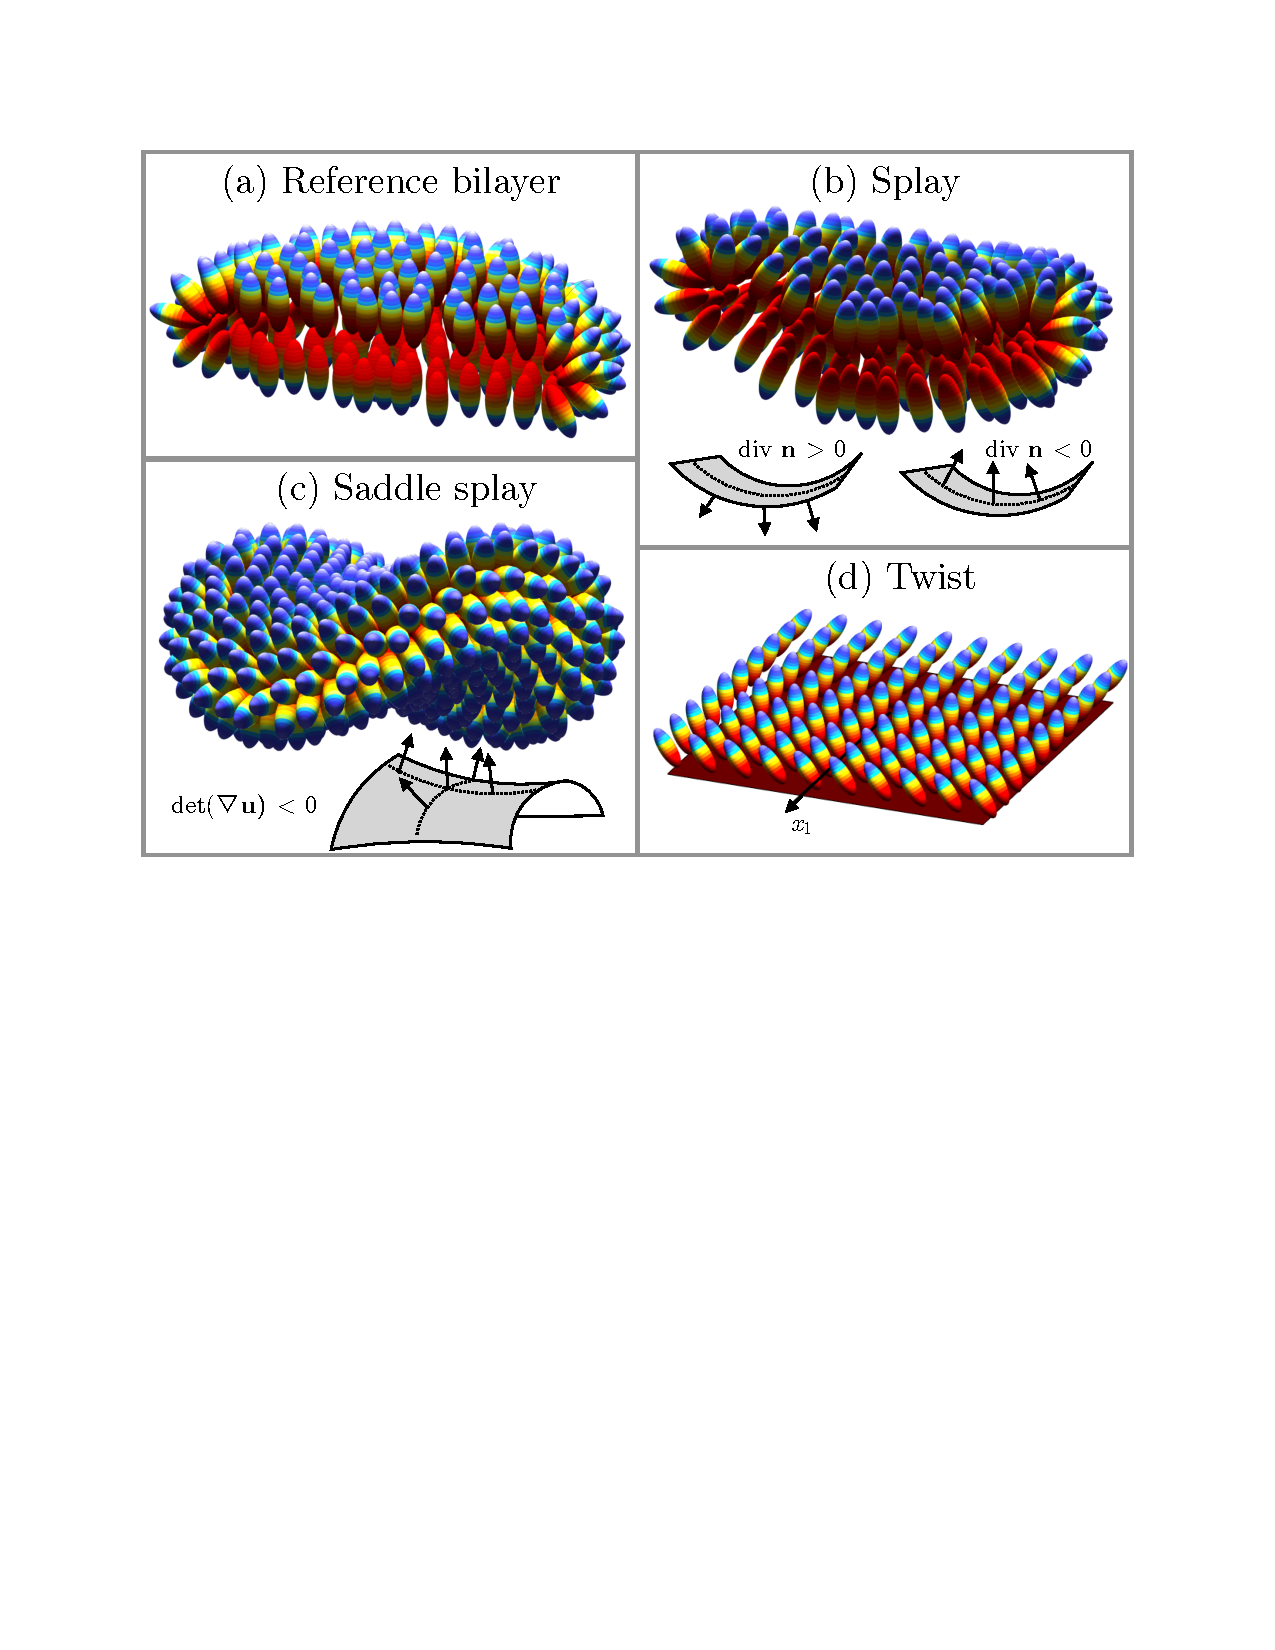
\includegraphics[width=0.46\textwidth]{Figures/Deformations.pdf}}
  \vspace{-5pt}
\caption{\label{fig:deformations} \footnotesize Sketch of the HK
 membrane model \cite{Hamm2000}.}
\end{wrapfigure}
%
This proposal will develop much-needed mathematical analysis to resolve
these controversies due to the assumptions in the HK theory. 


\sloppy
The HK framework assumes a three-dimensional lipid monolayer where the
internal structure consists of straight fibers that represent elongated
hydrocarbon chains.  The elastic energy density ${\cal W}$ is quadratic
in the Green-Lagrange strain tensor for this striated, internal
structure. This energy density decomposes into four, fundamental, and
independent deformations (Figure~\ref{fig:deformations}): splay ($\Div
{\bf n}$), twist ($\Curl {\bf n}$), saddle splay ($\det \nabla {\bf
n}$), and tilt ${\bf t}={\bf n}/({\bf N}\cdot {\bf n}) - {\bf N}$ where
${\bf N}$ is the unit surface normal;
\begin{equation}
\label{ansatz3}
{\cal W} \equiv \int_{\Sigma} 
  \tfrac{1}{2}\KB\left[ \left( \Div {\bf n} + k_0\right)^2 - k_0^2\right] 
+ \tfrac{1}{2}\KT (\Curl {\bf n})^2 + \KG  \det \nabla {\bf n} + \tfrac{1}{2}\KTH |{\bf t}|^2 \,dA.
\end{equation}
Here, the deformations come with elastic coefficients: the bending
modulus $\KB$, twist modulus $\KT$, saddle-splay modulus $\KG$, and tilt
modulus $\KTH$. The parameter $k_0$ is the spontaneous curvature and
determines the preferred lipid splay~\cite{RoLi15,Kozlov2007}.  

Although the HK elastic theory assumes small deformations, Galimzyanov
{\em et al.}~\cite{C9SM02079A} have shown that energies derived from
molecular dynamics and those derived from \eqref{ansatz3} are in
agreement, even when curvatures are large.  Under spatial scales much
larger than the membrane thickness, membrane energy is
well-characterized by the Canham-Helfrich energy used throughout the
fluid-structure literature \cite{QiangDu09, Lowengrub07,KimLai2010_JCP,
Hu, HuLaiSeolEtAl2016_JCP, qua-bir2014, qua-vee-you2019}. The
Canham-Helfrich energy is actually a special case of \eqref{ansatz3}
obtained by setting ${\bf n} =  \pm {\bf N}$ (the $\pm$ depending on
orientation) and collapsing both monolayers onto the membrane midplane.

\subsubsection{Simulations of the HAP model to estimate elastic moduli
and energy}
\begin{wrapfigure}[11]{r}{0.43\textwidth}
  \centerline{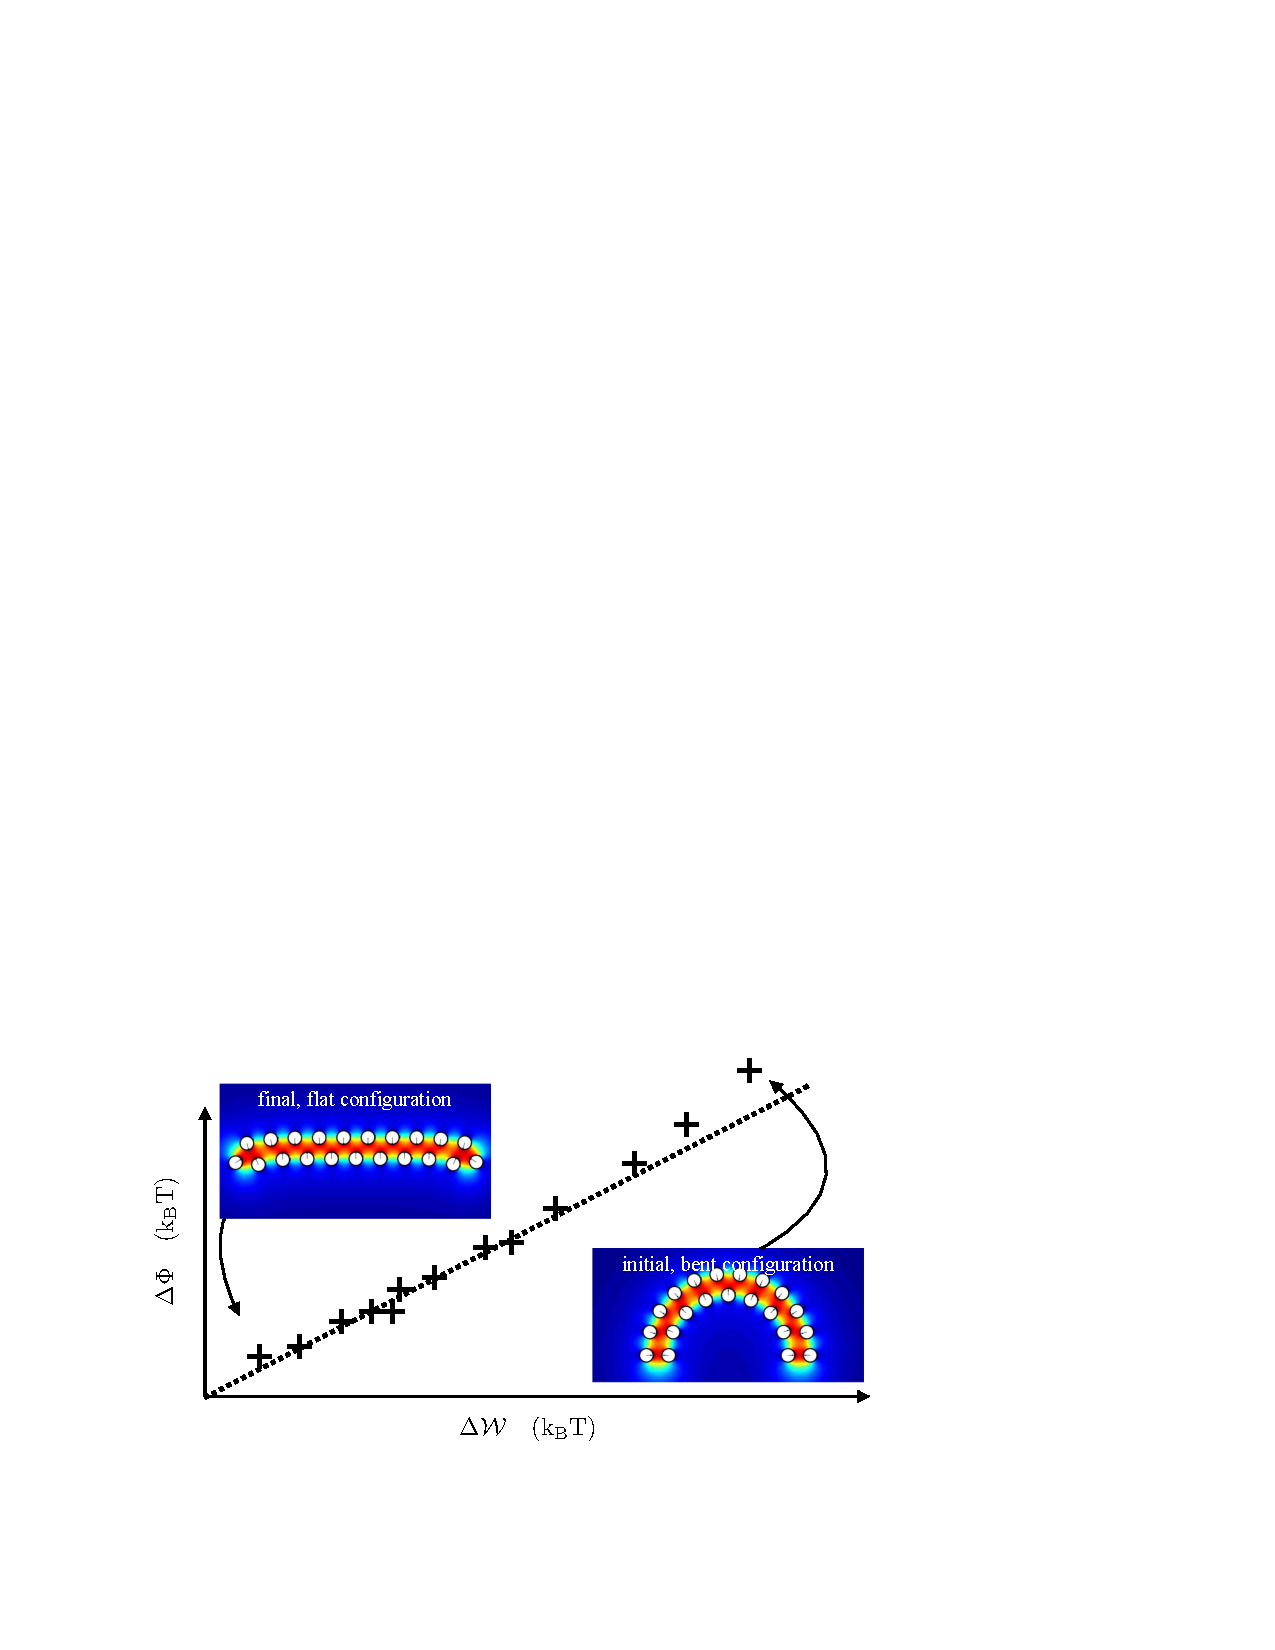
\includegraphics[width=0.42\textwidth]{Figures/Flattening.pdf}}
  \caption{\label{fig:flattening} \footnotesize Example of computing
  bending modulus of a lipid bilayer from particle simulation.}
\end{wrapfigure}
We propose to {\bf (i)} determine the value of effective elastic moduli
$\KB$, $\KT$, $\KG$, and $\KTH$ and then {\bf (ii)} understand how the
model parameters $\rho,$ $\gamma$, and the particle shape map onto
elastic moduli. An accurate and robust way to measure material
properties is to track the evolution of the bilayer as it relaxes from
an initially non-equilibrium
configuration~\cite{PhysRevLett.117.188102}.
Figure~\ref{fig:flattening} shows an example where the initial
configuration of a bilayer patch containing the splay deformation
without any other components (saddle splay, twist and tilt). As the bent
membrane flattens, both the self-interaction energy $\Phi$ and the
elastic energy ${\cal W}$ decrease, and because the saddle splay, twist,
and tilt stay zero, the slope gives the bending modulus in this case. 

Here we start with a particle-based bilayer in a specific
non-equilibrium shape that involves only one of the components of the
displacement in Figure~\ref{fig:deformations}, and then evolve the
particle system according to the time integration for \eqref{eq:stokes}.
Because elastic properties are independent of dissipation, we can forgo
solving for fluid velocity and set the translational velocity and
angular velocity directly proportional to the force and torque,
respectively. 

This yields a dissipation of the total potential \eqref{eq:total_poten},
which stabilizes the evolving bilayer shape. Therefore, we reconstruct
an evolving monolayer dividing surface $\Sigma$ and director field ${\bf
n}$ by interpolating the particle centers and orientations.
Using~\eqref{ansatz3}, we calculate a continuum energy $\mathcal{W}$
from the interpolated shapes.

We propose to conduct calculations similar to the example of
Figure~\ref{fig:flattening} for other elastic moduli such as the
effective twist modulus $\KT$.  Molecular dynamics investigations find a
twist modulus about 1 \kBT~\cite{LeVeWa14}, and here, the specific
non-equilibrium shape consists of a single layer of amphiphilic
particles on a hydrophobic substrate as illustrated by
Figure~\ref{fig:deformations}D. Having a nonzero twist requires nonzero
tilt because the surface gradient of the lipid director equals the
second fundamental form whenever tilt is zero locally. The twist
deformation is a fully three-dimensional deformation.
\S\ref{subsec:specific_aim_3} addresses outstanding implementation
issues like three-dimensional boundary integral equation solvers.

The gradient descent technique is ineffective for measuring the saddle
splay modulus $\KG$ because the saddle splay energy is largely invariant
under shape changes.  To evaluate $\KG$, we will combine the present
particle simulations with the string method from PI RR's work on
membrane fusion \cite{RyKlYaCo16}. The string method is a numerical
scheme that finds least energy pathways separating energy basins
\cite{doi:10.1063/1.2720838}.  In the simplified Canham-Helfrich
formulation, saddle splay energy is an exact indicator of topological
transitions, thanks to the  Gauss-Bonnet theorem \cite{TerziDeserno17}.
More generally, PI RR has shown that saddle splay acts as a topological
indicator even in the presence of nonzero tilt \cite{RyKlYaCo16}.  As a
result, saddle splay can be quantified from the transition energies of a
least energy path of pore formation (Figure~\ref{fig:saddle_splay}).

The field of membrane continuum mechanics still lacks consensus as to
whether HK energy is the appropriate functional for bilayer energy.
\textbf{(i)} Researchers have assumed that $\KT = 0$ to effect lateral
fluidity in membranes~\cite{Hamm2000, TerziDeserno17, C9SM02079A,
PhysRevE.102.042406}. A value $\KT = 0$, however, makes~\eqref{ansatz3}
a noncoercive functional. \textbf{(ii)} Recently,~\cite{TerziDeserno17}
derived a tilt curvature term that was neglected from the HK
analysis~\cite{Hamm2000}.  Later,~\cite{C9SM02079A}
and~\cite{PhysRevE.102.042406} independently identified an inconsistency
in the argument used by~\cite{TerziDeserno17} arising from a transversal
tilt invariance assumption.  In~\cite{RyKlYaCo16}, PI RR and
collaborators showed that the tilt vector leads to unphysical cusps
depending on how one accounts for membrane thickness.  \textbf{(iii)}
Theoretical analysis of lipid phase transitions predict a negative
saddle-splay modulus around $-8$ \kBT~\cite{SIEGEL2004366,
SIEGEL20085200} that gives rise to a larger energy barrier for monolayer
fusion than is found by experiments~\cite{FrRoPi17, Tran7106,
TerziDeserno17}.
\begin{wrapfigure}[11]{l}{0.32\textwidth}
  \centerline{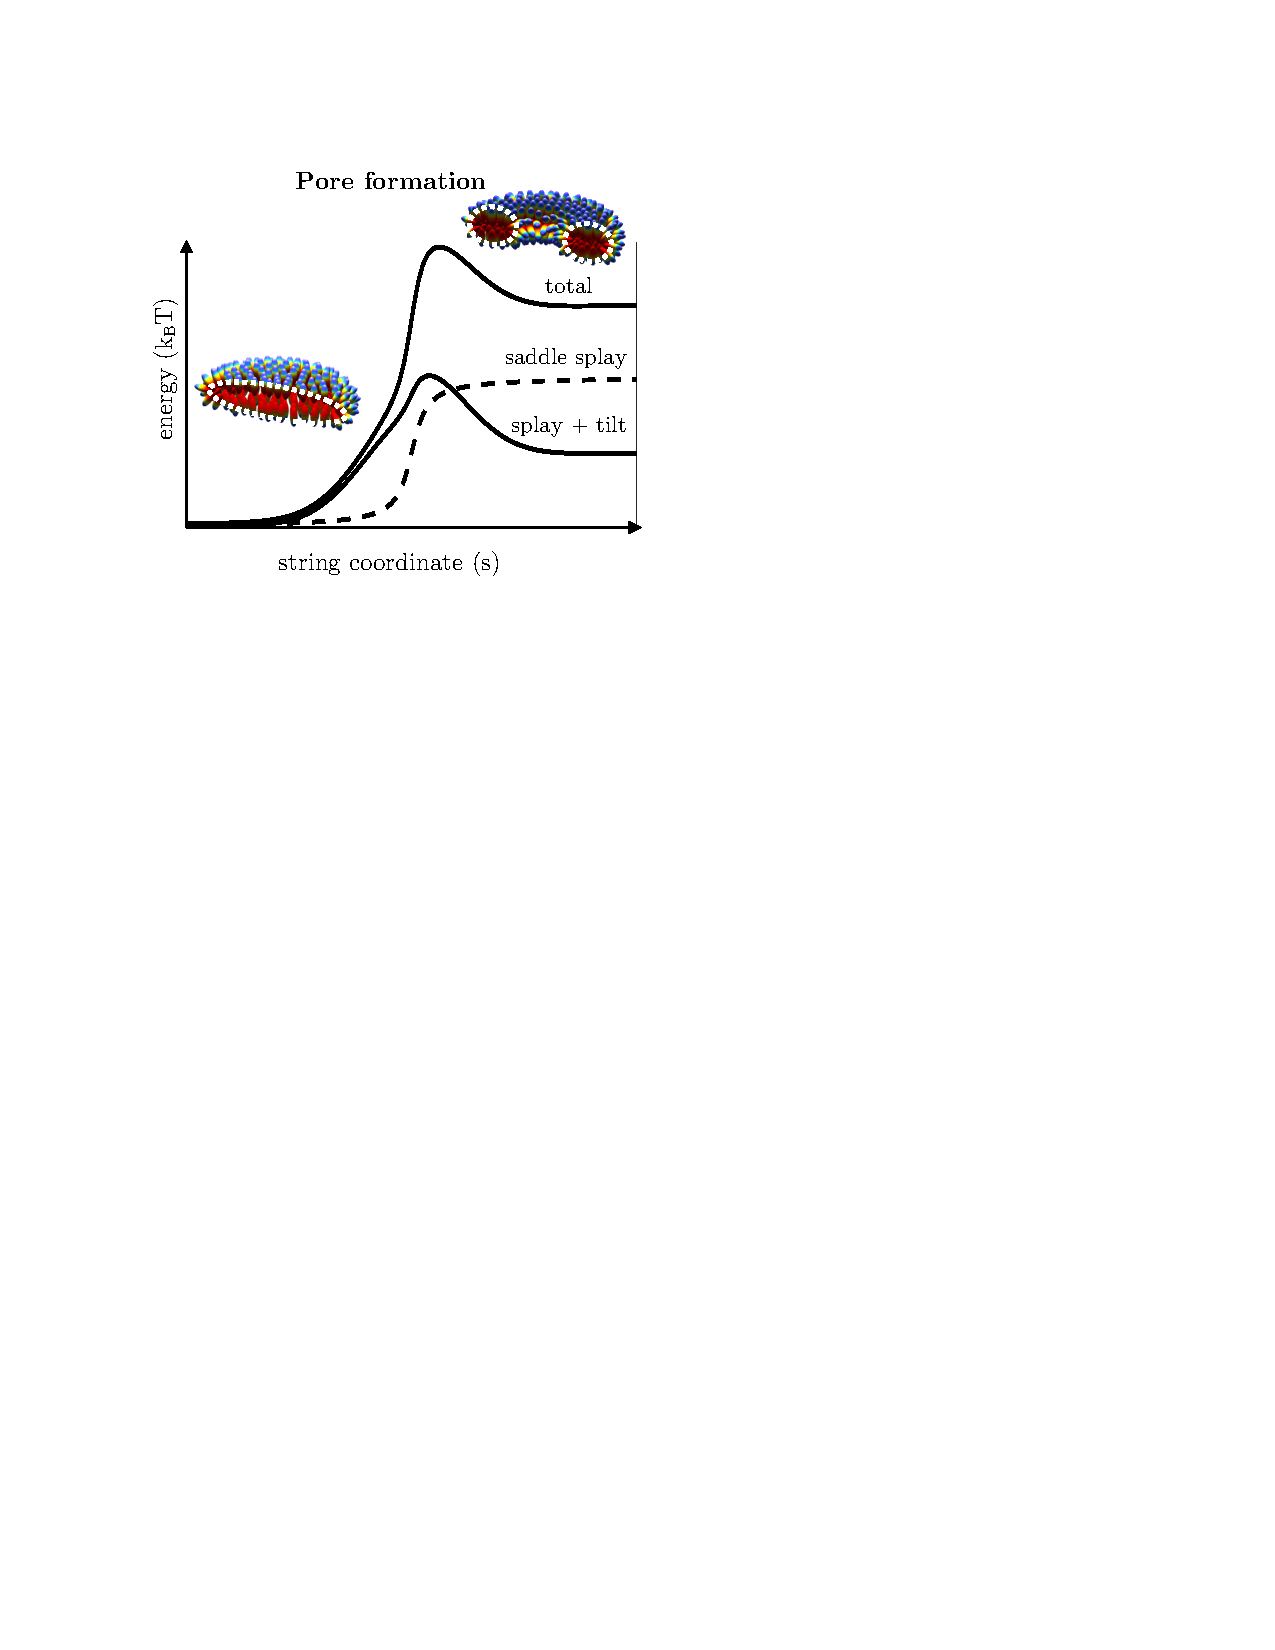
\includegraphics[width=0.31\textwidth]{Figures/SaddleSplayDiagram.pdf}}
  \caption{\label{fig:saddle_splay} \footnotesize Example of determining
  the saddle splay modulus.}
\end{wrapfigure}

The form of the elastic energy density~\eqref{ansatz3} is the same as
the Oseen-Frank energy density for nematic liquid
crystals~\cite{ANDRIENKO2018520, Tran7106, Helfrich73}. In fact, a lipid
monolayer acts as one layer in a smectic phase~\cite{REYESMATEO1995978,
Rangamani20140463, PhysRevLett.113.248102}. Based on this observation,
we propose to examine the HK analysis to resolve the aforementioned
inconsistencies. We will expand the strain tensor in terms of a plane
perpendicular to ${\bf n}$ (instead of the monolayer tangent plane as
done in the past works) so that the gradient terms in the elastic energy
completely decouple. Using this expansion we prove an exact identity
that gives the incompressibility condition by a Steiner-type polynomial
in $\Div {\bf n}$ and $\det \nabla {\bf n}$ \cite{Fe59}. In contrast,
the works~\cite{TerziDeserno17, PhysRevE.102.042406, Hamm2000,
C9SM02079A} utilize an approximate identity for incompressibility as a
base, so we can considerably improve upon the analysis of monolayer
energy.

\subsubsection{Analysis of the HAP model in terms of the HK functional}
The HK functional~\eqref{ansatz3} has transformed how scientists understand biological membranes, yet the
theory has received little attention in terms of
mathematical analysis. In the calculus of variations, the
principal question is whether a minimizer of an energy functional
exists. In the case of~\eqref{ansatz3}, the answer is presently unknown.
With regard to the simpler Canham-Helfrich energy,~\cite{Simon1993}
proved the existence of minimizing surfaces without boundary,
and~\cite{doi:10.1137/18M1195851} proved the well-posedness of a
spatially periodic, time-dependent elastic interface problem. An
analytical challenge for the HK functional~\eqref{ansatz3} is that
surface-director coupling makes it possible to have bounded energy
monolayers with corners, and such pathological examples must be ruled
out before carrying over the arguments for the Canham-Helfrich
functional to the present setting.

Our goal here is to develop tools that can explain functionals
like~\eqref{ansatz3} from first principles in terms of HAP. The
papers~\cite{doi:10.1063/5.0009734, Seguin2012, Seguin2014} give
statistical mechanical/mean field derivations of the Canham-Helfrich
energy from a pair-potential for rod-like molecules, but do not include
tilt, which is an indispensable deformation at biological scales. To
make progress, we must first understand how the HAP functional behaves
under various limits.

We first consider HAP in the limit of vanishing screening length. As a
concrete model problem, we consider a collection of colloidal polyhedral
where the binding energy of this system can be described by a discrete,
lower semicontinuous functional $\Phi_0$ whose value is the total
surface area of the polyhedra minus two times the area of any
overlapping faces. We conjecture that the $\Phi$ energy
$\Gamma$-converges to $\Phi_0$ \cite{Mugnai2013}, meaning that any
cluster points of minimizers of $\Phi$ converge to a minimum of $\Phi_0$
in the limit $\rho \to 0$. To address this conjecture, we employ
boundary layer analysis for the screened Laplace equation~\cite{Lee2018,
Lin2015, Shibata2004,1531-3492_2006_2_357, Lee2018}. The technique of
$\Gamma$-convergence is a powerful tool for numerical approximations and
with it we can help explain unexpected phenomena like hierarchical
self-assembly in colloidal systems~\cite{Luo2019}.

\end{comment}

